\chapter{Implemented software}

In order to test the feasibility and to try the speed of the different algorithms different software pieces were needed.

\begin{figure}[H]
\caption{Implemented acquisition software in the CERN infrastructure}
\centering
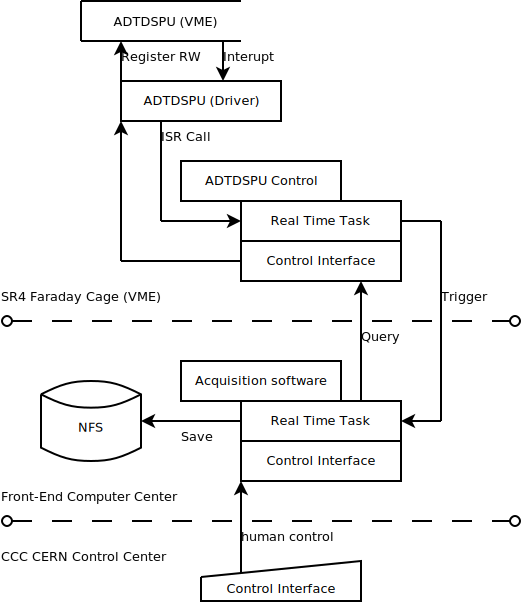
\includegraphics[scale=0.3]{ImplementedSoftFesa.pdf}
\end{figure}

The implemented system consist of three pieces of software~:
\begin{enumerate}
\item The software controlling the acquisition card in the machine.
\item An acquisition software that runs on a standard front-end Linux machine that is taking data during the \glspl{MD}.
\item And an analyzing software that can compute the \glspl{FFT} on \glspl{GPU}.
\end{enumerate}

In the final version the software will be merged in a single executable that should run on the machine with the \gls{GPU} and the receiver card. The present solution has been put into place because the present hardware is still in development and there is no way of acquiring the maximum of 2880 bunches from the machine. The hardware is receiving the acquisition data but the \gls{VME} is not fast enough to transfer it to the \gls{CPU}.

\section{ADTDSPU control software}

The first layer that was needed is a driver that can control the \gls{VME} card and forward the interrupts. This is done using the standard driver framework from the \gls{CO} at \gls{CERN}.

The standard \gls{FESA}, the standard middle-ware framework used at \gls{CERN} to control equipments, was used to develop a higher level software to control the card. This particular card needs a real time task in order to react to an interrupt coming from the hardware and to inform when a new acquisition is ready to be read.

The software was originally written by David Gl{\'e}nat, Andrey Pashnin took it over and wrote the specific part of the ``tune acquisition'' and is now under Fr{\'e}d{\'e}ric Dubouchet responsibility as all \gls{ADT} software.

It is made of tree main part, two of them are interface with the user. The tune measurement control interface is there to set the acquisition parameters. The Tune measurement data is there to receive the data from the card to the user. Finally a real-time task it there to receive the interrupt and notify the user that there is new data available.

The Interfaces are exposed trough the \gls{CERN} middle-ware so it is available from other application as the data acquisition software.

\subsection{Control interfaces}

This interface is basic it allow the user to set the register to enable the acquisition and to set the mask that decide witch bunches in the acquisition have to be recorded in the memory. The mask is described as an array of 3564 short (2-bytes word) that can be either 0 (not selected) or 1 (selected).

This interface allow us to select witch bunch we want to acquire, of course the machine can never be fully saturated by bunches, because you need an abort-gap in the machine to allow the extraction kicker to extract the beam.

Even if the present interface allow us to have the full bunches of the machine selected. It has been very clear that as the memory is limited to 16 kilo-short (32 kilo-bytes) we would have too many interrupts per second for the interface to be usable.

There is also two other problems that this interface is facing, there is no double buffering so as the CPU is reading the values new incoming values would be lost, also the \gls{VME} is too slow to support the rate at witch data is coming.

The data interface is the interface the data acquisition software is using. It allows to get the values back from the memory in the \gls{CPU} as soon as they become available. It uses a system call subscription where the interface notify the client software that new data has become available (more about this in the section~\ref{sec:obs_mem_acq}).

It can also give a read back from the hardware of the various parameters we set from the tune measurement control interface~: the mask and all the controls.

\subsection{Observation memory acquisition}
\label{sec:obs_mem_acq}

\begin{figure}[H]
\caption{ADTDSPU tune acquisition process description}
\centering
\includegraphics[scale=0.3]{adtdspu_acq.pdf}
\end{figure}

A ``real-time'' process is waiting for the interrupt to happen, using a select like mechanism. The Linux used at \gls{CERN} on the front-ends is a custom kernel with the real-time patch, this guarantees that the latency between the interrupt and the process being called is not too big (usually under 10 micro-seconds).

This process create a custom event sources that trigger the copy of the hardware buffer into the \gls{CPU} buffer and notify the tune measurement data task that the buffers are ready to be read.

Notifying the task actually call it and this task (called server task as this is an interface task) is then telling its clients to come and get the acquisition data. 

\section{Acquisition software}

The acquisition software was used to check that the idea of getting the tune out of the DSPU card data was feasible as well as providing a means to log the acquisition to a file for subsequent checking and processing.

\begin{figure}[H]
\caption{ADTDSPU tune acquisition software interface in the FESA framework}
\centering
\includegraphics[scale=0.25]{amplitude_log.pdf}
\label{fig:tuneacq}
\end{figure}

The acquisition software uses the \gls{CMW}, a library used at \gls{CERN} to communicate between different layers of the accelerators control software, to connect to the \gls{ADTDSPU} control software and get the data when they are published (at the time of interrupt).

The acquisition software is then able to compute the \gls{FFT} using \gls{FFTW} and display it to the operators in the \gls{CCC} from where all the eight accelerators of \gls{CERN} are controlled. On the interface one can decide which type of graph to display and also enable saving the data files to be processed by the data analysis software.

\subsection{Control interface}

\subsection{ADTDSPU subscription}

\begin{figure}[H]
\caption{Tune measurement acquisition software in the FESA framework}
\centering
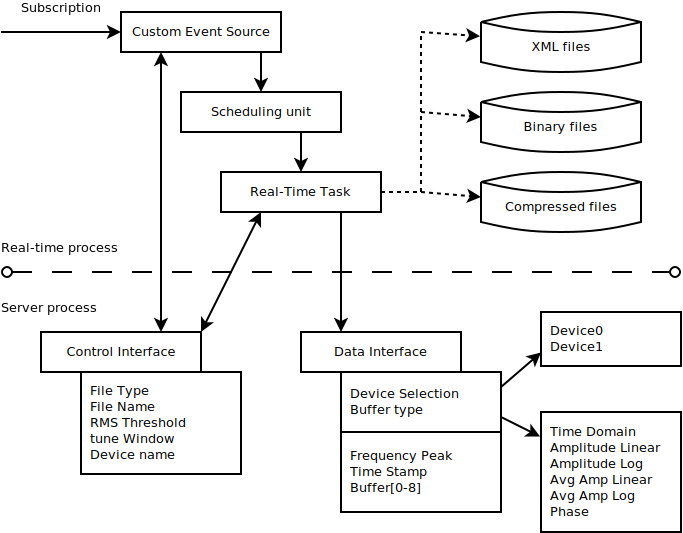
\includegraphics[scale=0.3]{tune_meas.pdf}
\end{figure}

\section{Data analysis software}
\label{sec:data_analysis_software}

The data analysis software is a set of modules that can be enabled or bypassed to test the usefulness of an algorithm. The modularity of the data analysis software allow us to check the time taken by each part of the algorithm and validate it against the constraints.

\begin{figure}[H]
\caption{Time f\/low with different implementations and with 3000 bunches of 2048 points each.}
\centering
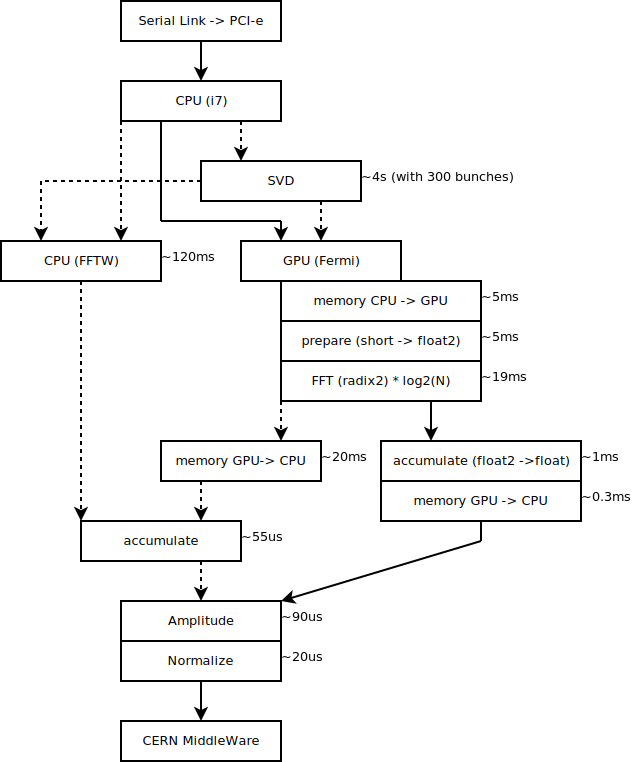
\includegraphics[scale=0.3]{PC-flow.pdf}
\label{fig:PCFlow}
\end{figure}

The data is first loaded from the files that were written by the acquisition software. Then it is filtered by a notch filter as described in the notch section~\ref{sec:notch}. And finally to the different algorithms as shown in the figure~\ref{fig:PCFlow}.

The first optional step is to apply a \gls{SVD} as described as suggested by Rama Calaga~\cite{PhysRevSTAB.7.042801} and by Wolfgang H{\"o}f\/le\cite{HofleChamonix12} which should reduce the noise in the signal (results are shown in section~\ref{sec:SVD}).

The \gls{FFT} are either computed on a \gls{GPU} or the \gls{CPU}, One could actually use \gls{OpenCL} on the \gls{CPU} and test the whole \gls{OpenCL} path. The different paths are due to memory copying, in the case of computations on the \gls{GPU}, one has to move the data from the \gls{CPU} central memory to the \gls{GPU} memory. This will be described in section~\ref{sec:FFT}.

To have a clear image and to combine the real and imaginary part of the \gls{FFT} we use the amplitude. It has been validated in the acquisition software as been the best metric, but could be changed at will in the final version. The amplitude is described in section~\ref{sec:amplitude}.

The accumulation over all theses bunches is done, which will give an average spectrum.

The normalization step is only present for displaying the spectrogram (see section~\ref{sec:spectrogram}) and will not be needed for the final version.
